\section{Variantendiskussion}
\label{sec:Variantendiskussion}
In der Entwurfsphase sollen aus den Anforderungen der Analysephase Modelle der zu entwickelten Software entstehen, die die konkreten Hardware- und Softwarebezogenen Anforderungen berücksichtigen. Diese Modelle gelten dann als unmittelbare Vorlage für die sich anschließende Implementationsphase. (vgl. \cite[S. 69]{dumke-2003})

Zu Beginn soll eine Marktrecherche durchgeführt werden, um bestehende Lösungen zu analysieren und auf Eignung zu Prüfen. Mit den gewonnen Erkenntnissen soll dann abgewägt werden ob Standartsoftware beschafft werden kann oder eine eigenentwicklung Veranlasst wird.
%Das erfolgt im Rahmen einer Variantendiskussion, in der verschiedene Ansätze und Technologien zur Umsetzung der Software bewertet werden.

Letztendlich soll der Programm- und Datenentwurf mithilfe geeigneter Modelle erarbeitet werden. Dies umfasst die Festlegung der Softwarearchitektur, der Datenstruktur sowie etwaiger Schnittstellen und der grafische Oberfläche.

\subsection{Marktrecherche}
\label{sec:Marktrecherche}
Im Rahmen der Marktanalyse wurden drei verschiedene Softwarelösungen für die Anwesenheitsplanung verglichen. Das Ziel dieser Analyse war es, Akquisitionsoptionen für das geplante Softwareprojekt zu ermitteln. Um Entscheidungen über die Eignung treffen zu können, wurden die Softwareprodukte auf den Erfüllungsgrad der Anforderungen geprüft. Dafür wurde eine Bewertungsmatrix erstellt, die funktionale- als auch nichtfunktionale Anforderungen beinhaltete. Dabei wurden die Kriterien so gewählt und gewichtet das zwingend erforderliche Anforderungen höher gewichtet wurden als optionale Anforderungen.

%TODO:Tabelle muss ordentlich Platziert werden
\begin{figure}[htb]
    \centering
    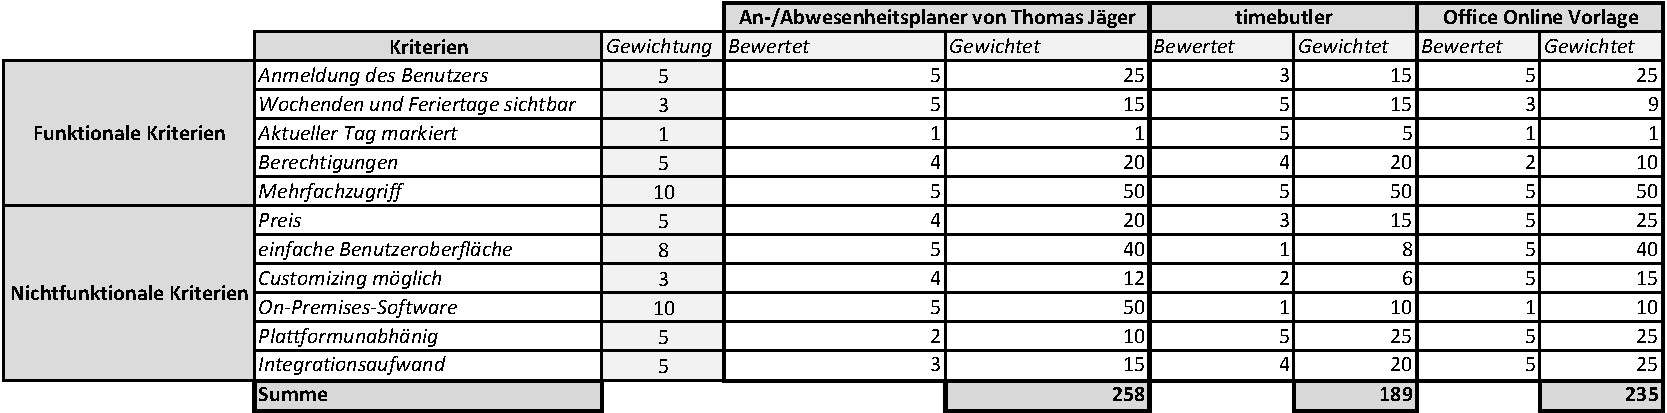
\includegraphics[width=0.9\textwidth,angle=0]{abb/Markterkundung.pdf}
    \caption[Beschreibung]{ Tabelle Markterkundung}
    \label{tab:Markterkundung}
\end{figure}

\subsubsection{An-/Abwesenheitsplaner von Thomas Jäger}
\label{sec:AnAbwesenheitsplaner}
Die erste betrachtete Software, der An-/Abwesenheitsplaner von Thomas Jäger, zeichnete sich durch die besonders intuitive Benutzeroberfläche aus. Bei der Betrachtung der anderen funktionalen Kriterien wurde festgestellt, dass die Software alle benötigten Anforderungen erfüllt und damit für den Einsatz geeignet ist. Negativ zu bewerten ist allerding, das die Software nur als Windows Programm zur Verfügung steht und damit nicht Plattformunabhängig eingesetzt werden kann. Zudem müsste ein solches Programm auf jedem Client PC im SMK installiert werden um die Software für alle Nutzbar zu machen. Damit ergibt sich ein hoher initialer Integrationsaufwand und auch späterer Wartungsaufwand den es zu berücksichtigen gilt. (vgl. \cite{AnAbwesenPlaner})


%Die Benutzerfreundlichkeit wurde jedoch als etwas komplex und steil eingestuft, was eine gewisse Einarbeitungszeit erforderte. Zudem war der Support nur eingeschränkt verfügbar und die Preisgestaltung vergleichsweise hoch. (vgl. \cite{AnAbwesenPlaner})
\subsubsection{timebutler}
\label{sec:timebutler}
Das zweite Programm namens timebutler überzeugte hingegen durch seine Plattformunabhängigkeit. Damit könnte es ohne großen Integrationsaufwand im SMK eingeführt und betrieben werden. Die Software bietet alle geforderten Funktionalitäten hat jedoch eine komplizierte Benutzeroberfläche und stellt viele Funktionen bereit die nicht benötigt werden. Das resultiert in höheren Anschaffungskosten als bei dem An-/Abwesenheitsplaner von Thomas Jäger. Besonders negativ ist zu bewerten, dass die Software zwar Plattformunabhängig ist, da sie auf Webtechnologien aufbaut, jedoch nicht als On-Premises-Software verfügbar ist. Damit müsste auf die Cloud des Anbieters zurückgegriffen werden was nicht gewünscht ist. (vgl. \cite{timebutler})

\subsubsection{Online Office Datei}
\label{sec:OnlineOffice}
Die dritte betrachtete Lösung ist die Verwendung einer Online Tabellenkalkulations Vorlage. Das würde es ermöglichen, die bereits vorhandenen Excel Tabellen für die Anwesenheitsplanung weiter zu verwenden. Durch das zurückgreifen auf Online Funktionalitäten die \zB von Microsoft mit Office356 oder mit Onlyoffice in Verbindung mit Nextcloud zur Verfügung stehen, kann man den gleichzeitigen Zugriff auf diese Listern erreichen. Damit würde man das Hauptproblem der einfachen Excel Dateien lösen. Doch auch hier müsste man im Falle des einsatzes von Office356 auf die Microsoft Cloud zurückgreifen. Desweiteren gibt es nur begrenzte Möglichkeit diese Excel Listen vor ungewollter Änderungen zu schützen und ein Berechtigungskonzept durchzusetzten.

\subsubsection{Auswertung der Marktrecherche}
\label{sec:AuswertungMarktrecherche}
Nach Betrachtung der drei Programme wurde festgestellt, dass keines der drei für eine Akquisition in frage kommt, da jedes seine individuellen Schwachstellen mit sich bringt. Der An-/Abwesenheitsplaner von Thomas Jäger wäre von allen die beste Option, da es eine benutzerfreundliche Oberfläche, eine solide Funktionalität und eine angemessene Preisgestaltung vereint. Die Plattformunabhängigkeit ist jedoch im SMK ein großer Faktor, da sich das neue Programm möglichst gut in die vorhandene Infrastruktur einfügen soll. Deswegen wurde sich gegen eine Akquisition von Standartsoftware entschieden. Um die geforderten Funktionalitäten abzubilden ohne dabei die Schwachstellen der Analysierten Programme inkauf nehmen zu müssen wurde ich für eine Eigenentwicklung der Software entschieden.

\subsection{Eigenentwicklung}
\label{sec:Eigenentwicklung}
Für die Umsetzung wurde Referat 12 mit der Entwicklung der Softwarelösung beauftragt. Die benötigten Hard- und Softwareressourcen vom SMK bereitgestellt und der zeitliche Rahmen für das Projekt wurde mit 32 Arbeitstagen angesetzt. Die genaue Aufschlüsselung des Projektablaufes siehe \ref{abb:Gantt}.

Für die Entwicklung der Software sethen dem Entwickler ein voll ausgestatteter Arbeitsplatz, sowie mehrere virtuelle Maschinen im Rechenzentrum zur Verfügung. Damit hat der Entwickler freie Hand bei der Umsetzung. Zu beachten ist jedoch, dass nach Möglichkeit auf die bestehende Infrastruktur zurückgegriffen bzw. berücksichtigt wird.


\subsection{Umsetzungsvarianten}
\label{sec:Umsetzungsvarianten}
Nach der Analyse der Anforderungen und der Markterkundung sollen in diesem Abschnitt verschiedene Umsetzungsvarianten diskutiert werden. Es gibt verschiedene Softwareentwicklungsansätze, die für dieses Projekt gewählt werden können.

Die simpelste Variante ist die Entwicklung einer monolithischen Anwendung, die als Programm auf den Clients installiert wird. Hierbei stellt das Programm alle nötigen Komponenten und Dienste im ganzen bereit. Dieser Ansatz kann gut geeignet sein, wenn die so entwickelte Anwendung auf einer bestimmten Plattform ausgeführt werden soll und keine Notwendigkeit für eine verteilte Architektur besteht. Da das Programm bei einer monolithischen Architektur sowohl das User-Interface als auch die Logik beinhaltet wird kein extra Server dafür benötigt.

Für den Anwesenheitsplaner könnte auch auf die Client-Server-Architektur gesetzt werden, die klassisch bei Webbasierten Anwendung mit Backend-Server und einer Datenbank eingesetzt wird. Bei dieser Art von Anwendung werden die Funktionen auf mehrere Schichten aufgeteilt. Der Backend-Server kümmert sich um die Verarbeitung der Anfragen und die Bereitstellung von Daten, während die Datenbank die persistenten Speicherung der Informationen ermöglicht. Das bedeutet zwar mehr Integrationsaufwand, würde aber eine gute Flexibilität bieten und wäre durch den Einsatz von Webtechnologienenn Zukunftssicher da die Anwendung Plattformunabhängig eingesetzt werden kann. Die potenziellen Nachteile wie die ständige Netzwerkabhängigkeit der Clients um den Dienst zu Nutzen, können im Anwendungskontext vernachlässigt werden.

Auf grundlage der Anforderungen solle auf eine Client-Server-Architektur mit Frontend und Backend gesetzt werden. Der etwas höhere Integrationsaufwand dieser Architektur wird durch die dabei entstehend Vorteile ausgeglichen. Die Integration einer monolithischen Architektur würde im konkreten Fall ebenfalls einen höheren Aufwand ergeben als vorgesehen, da für mehrere Plattformen entwickelt werden müsste. Desweiteren sind im SMK bereits viele der für eine Client-Server-Architektur geforderten Systeme vorhanden, da es eine oft eingesetzte Architektur ist. Somit können diese Ressourcen genutzt werden.



\subsection{Programm und Datenentwurf}
\label{sec:ProgrammUDatenentwurf}